	\begin{myex}
		La fonction $f(x) = -x + 1$ est décroissante sur $\intervOO{- \infty }{+ \infty}$.
		\begin{center}
			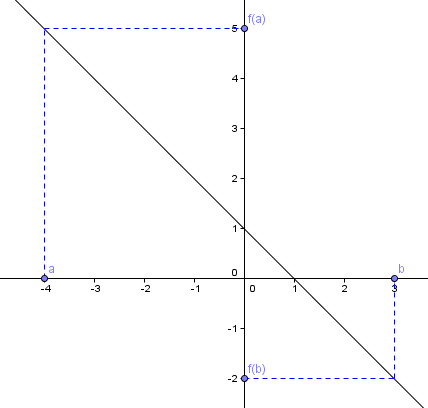
\includegraphics[scale=0.65]{./img/decroiss}
		\end{center}
		
		\begin{itemize}
			\item $a$ et $b$ appartiennent à $\intervOO{- \infty }{+ \infty}$, on a $a \leq b$ donc $f(a) \geq f(b)$.
			
			\item $-4 \leq 3$ donc $f(-4) \geq f(3)$ ($5 \geq -2 $).
		\end{itemize}
		
	\end{myex}